\vspace{-5pt}

\section{Overview}
\label{sec:overview}

We introduce verification in FCSL by informally explaining a
fine-grained concurrent program for computing in place a spanning tree
of a binary directed graph~\cite{Hobor-Villard:POPL13,Raad-al:colosl}.

{
\setlength{\belowcaptionskip}{-10pt} 
\begin{figure}
\centering
{\small{
\[
\begin{array}{rl}
\Num{1} & \esc{span}~(x : \tp{ptr}) : \tp{bool}~\{ 
\\ 
\Num{2} & ~~~~ \kw{if}~~x~\esc{==}~\esc{null}~~\kw{then}~~\kw{return}~\esc{false};    
\\
\Num{3} & ~~~~ \kw{else} \\
\Num{4} & ~~~~ ~~~~ b \Asgn \esc{CAS}(x\esc{->}m, 0, 1); \\ 
\Num{5} &~~~~  ~~~~ \kw{if}~~b~~\kw{then} \\
\Num{6} & ~~~~ ~~~~ ~~~~ (r_l, r_r) \Asgn(\esc{span}(x\esc{->}l)~||~\esc{span}(x\esc{->}r)); \\
\Num{7} & ~~~~ ~~~~ ~~~~ \kw{if}~~\neg{}r_l~~\kw{then}~~x\esc{->}l~\esc{:=}~\esc{null};  \\
\Num{8} & ~~~~ ~~~~ ~~~~ \kw{if}~~\neg{}r_r~~\kw{then}~~x\esc{->}r~\esc{:=}~\esc{null};  \\
\Num{9} & ~~~~ ~~~~ ~~~~ \kw{return}~\esc{true};\\
\Num{10} & ~~~~ ~~~~ \kw{else}~~\kw{return}~\esc{false}; \}
\end{array}
\]
\vspace{-3pt}  
}}
\caption{Concurrent spanning tree construction procedure.}
\label{fig:span}
\end{figure} 
}

\subsection{A Graph Spanning Tree Algorithm and its Intuition}
\label{sec:algorithm}


The recursive procedure \code{span} (Figure~\ref{fig:span}) takes an
argument $x$, which is a pointer to a node in the graph, and constructs
the spanning tree rooted in $x$ by traversing the graph and removing
redundant edges.
%
The graph is implemented as a memory region where each pointer's
target value is a triple. The triple's first component is a bit $m$
indicating whether the node is \emph{marked}; the second and third
components are pointers to the node's \emph{left} and \emph{right}
successors, or~\code{null} if a successor doesn't exist.

{
\setlength{\belowcaptionskip}{-10pt} 
\begin{figure*}[t]
\centering
\ifdefined\psflag
    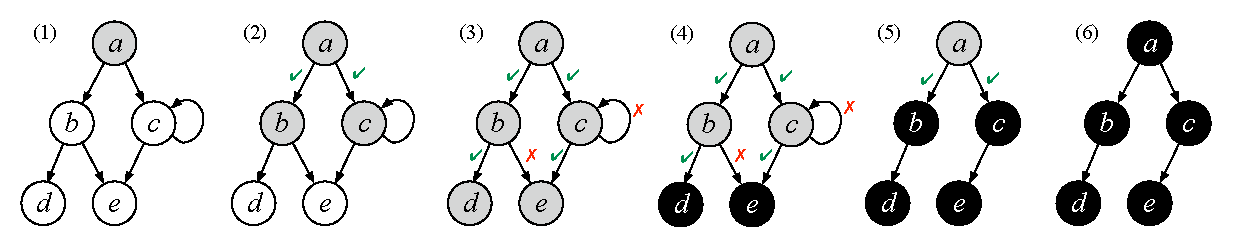
\includegraphics[width=0.95\textwidth]{stages.eps}
\else
    \includegraphics[width=0.95\textwidth]{stages-eps-converted-to.pdf}
\fi
\caption{Stages of concurrent spanning tree construction. A node is
  painted grey right after a corresponding thread successfully marks
  it (line~4 of Figure~\ref{fig:span}). It is painted black right
  before the thread returns \texttt{true} (line~9). A black subtree is
  \emph{logically ascribed} to a thread that marked its
  root. \textcolor{OliveGreen}{\cmark} indicates a child thread
  exploring an edge and succeeding in marking its target node;
  \textcolor{red}{\xmark} indicates a thread that failed to do
  so. (1)~the main thread marks $a$ and forks two children; (2)~the
  children succeed in marking~$b$ and~$c$; (3)~only one thread
  succeeds in marking~$e$; (4)~the processing of~$d$ and~$e$ is done;
  (5)~the redundant edges $b \rightarrow e$ and $c \rightarrow c$ are
  removed by the corresponding parent threads; (6)~the initial thread joins
  its children and terminates.}
\label{fig:stages}
\end{figure*}
}

If $x$ is \code{null}, \code{span} returns \code{false}
(line~2). Otherwise, it tries to mark the node by invoking the
compare-and-swap (CAS) operation (line~4). If \code{CAS} fails, then
$x$ was previously marked, \ie included in the spanning tree by
another call to \code{span}, so no need to continue (line~10). If
\code{CAS} succeeds, two new parallel threads are spawned (line~6):
\code{span} is called recursively on the left ($x.l$) and right
($x.r$) successors of $x$, returning respectively the booleans $r_l$
and $r_r$ upon termination. When $r_l$ is \code{false}, $x.l$ has
already been marked, \ie, \code{span} has already found a spanning
subtree that includes $x.l$ but doesn't traverse the edge from $x$ to
$x.l$. That edge is superfluous, and thus removed by nullifying $x.l$
(line~7). The behavior is dual for $x.r$. Figure~\ref{fig:stages}
illustrates a possible execution of~\code{span}.

% \begin{comment}
% Why is \code{span} memory-safe? Assume that the initial heap
% implements the binary graph, and that the heap is modified only by
% calls to \code{span}, and no other interference is allowed. Then the
% algorithm is memory safe, because each node reachable from the graph's
% root will be marked via \code{CAS} (line~4) by exactly one thread (and
% the nodes are never un-marked). The same thread that marks the node
% $x$ will remove the redundant edges to $x.l$ and $x.r$, if it
% discovers that these successor nodes have been previously marked. At
% any rate, it can never happen that a non-existent pointer is
% dereferenced, or that a pointer is dereferenced which doesn't store a
% triple containing a marked bit, and the left and right successor.
% %
% Figure~\ref{fig:stages} illustrates a possible execution
% of~\code{span}. \an{Hmm, a lot of discussion to simply say that at the
%   end we didn't read bad stuff. The paragraph seems superfluous.}
% \end{comment}

Why does \code{span} compute a {\em tree}? Assume that
\hypertarget{asm1}{{(1)}} the graph initially represented in memory is
{\em connected}, and that \hypertarget{asm2}{{(2)}} it is modified
only by recursive calls to \code{span}, with no external
interference. To see that \code{span} obtains a tree, consider four
cases, according to the values of $r_l$ and $r_r$. If
$r_l\,{=}\,r_r\,{=}\,\mathtt{\small{true}}$, then the calls to
\code{span} have, by recursive assumption, computed trees from
subgraphs rooted at $x.l$ and $x.r$ to trees. These trees have
disjoint nodes, and there are no edges connecting them. As will be
shown in Section~\ref{sec:devel}, this will follow from a property
that each tree is {\em maximal} \wrt the resulting \emph{final}
graph's topology (\ie, the tree cannot be extended with additional
nodes).  Lines~7 and~8 of \Code{span} preserve the edges from $x$ to
$x.l$ and $x.r$; thus $x$ becomes a root of a tree with subtrees
pointed to by $x.l$ and $x.r$ (Figure~\ref{fig:stages}(6)). If
$r_l\,{=}\,\mathtt{\small{true}}$ and
$r_r\,{=}\,\mathtt{\small{false}}$, the recursive call has computed a
tree from the subgraph rooted at $x.l$, but $x.r$ has been found
marked. The edge to $x.r$ is removed in line~8, but that to $x.l$ is
preserved in line~7; $x$ becomes a root of a tree with left subtree
rooted in $x.l$, and right subtree empty
(Figure~\ref{fig:stages}(5)). The case
$r_l\,{=}\,\mathtt{\small{false}}$, $r_r\,{=}\,\mathtt{\small{true}}$
is dual. The case $r_l\,{=}\,r_r\,{=}\,\mathtt{\small{false}}$ results
in a subtree containing just the root $x$
(Figure~\ref{fig:stages}(4)).

Why does \code{span} construct a \emph{spanning} tree? Consider the
{\em front} of the constructed tree in the initial graph (\ie, the
nodes immediately reachable in the initial graph, from the nodes of
the constructed tree. For example, in Figure~\ref{fig:stages}(5), the
front of $b$ are nodes $d, e$ in Figure~\ref{fig:stages}(1)). We will
show in the next section that this front must contain only marked
nodes, as otherwise \Code{span} would have proceeded with node
marking, instead of terminating. Thus the front of the tree
constructed by the top-level call to \code{span} must be
included in the very same tree. Otherwise, there exists a node which
is marked but not in the tree. Therefore, this node must have been
marked by another thread, thus contradicting assumption
\hyperlink{asm2}{(2)}. Since, by \hyperlink{asm1}{(1)}, the initial
graph is connected, a tree which contains its front must contain all
the nodes, and thus be a spanning~one.


\subsection{Infrastructure for Mechanizing the Proof in FCSL}
\label{sec:inform-proof-devel}

To flesh out the above informal argument and mechanize it in FCSL, we
require a number of logical concepts. We describe these next, and tie
them to the \code{span} algorithm.

%While the described informal argument of the algorithm's full
%funcional correctness is morally sound, it omits a number of important
%aspects, which should be taken into the account while building a
%rigorous proof. We will now outline these components of the formal
%development. \ab{This para needs strengthening. Can we remind the
%  reader that we have motivated the need for formal verification in
%  Sect. 1 and now we are going to follow (1) -- (4) (are we? as far as
%  I understand, that's the intention, looking at the paragraph
%  headings.)}

\subsubsection{Concurroids}
\label{sec:conc-graph-prot}

FCSL requires an explicit description of the common assumptions that
threads operating on the shared resource observe. Such agreement
between threads is needed so that one thread's changes match other
threads' expectations. In the case of \Code{span}, for example, one
assumption we elided above is that an edge out of a node $x$ can be
removed only by a thread that marked $x$. This thread can rely on the
property that edges to $x.l$ and $x.r$ won't be nullified by another
thread. These assumptions are formalized by STSs of a special form,
which are called \emph{concurroids}.

%We next describe these STSs in general, and illustrate with the STS
%for \Code{span}.

The state of each concurroid is divided into three components
$[\mathit{self}~|~\mathit{joint}~|~\mathit{other}]$. The \emph{joint}
component describes shared state that all threads can change. The
\emph{self} and \emph{other} components are \emph{owned} by the
observing thread, and its environment, respectively, and may be
changed only by its owner. If there are two threads $t_1$ and $t_2$
operating over a state, the proof of $t_1$ will refer by \emph{self}
to the private state of $t_1$, and by \emph{other} to the private
state of $t_2$, and the roles are reversed for $t_2$.
%In the specification and proofs, however, it may use the \emph{other}
%component, if it is needed to express some properties of interest.
This thread-specific, aka.~\emph{subjective}, split into \emph{self},
\emph{joint} and \emph{other} is essential for making the proofs
insensitive to the number of threads forked by the global program, and
the order in which this is done~\cite{LeyWild-Nanevski:POPL13}. We
also note that the \emph{self} and \emph{other} components have to be
elements of a PCM, \ie, a set $\pcmS$ with an associative and
commutative \emph{join} operation $\pcmF$, and a unit element $\pcmU$.
%
PCMs enable general and compositional representation of thread-owned
state (auxiliary or real), which can be split between parallel
threads~\cite{LeyWild-Nanevski:POPL13}. Intuitively, commutativity and
associativity account for those of a parallel composition of threads,
and partiality captures the fact that not all splits/combinations of
state are valid.

All three state components of a concurroid may contain real state, \ie
heap, or \emph{auxiliary state}~\cite{Lucas:TR,Owicki-Gries:CACM76},
which is kept for logical specification, but is erased before
execution.
%
In the case of the \code{span} procedure, the \emph{joint} component
is the heap encoding the graph to be spanned, as described above.
%
%Every pointer $x$ in this heap represents a node. It points to a
%triple $(m, l, r)$, defining the marked bit $m$ of the node $x$, and
%pointers $l$ and $r$ to the left and right successor of $x$.
%
The \emph{self} and \emph{other} components are auxiliary state,
consisting of sets of nodes (\ie, pointers) marked by the observing
thread and its environment, respectively. These components are
elements of a PCM of sets with disjoint union $\dotcup$ as~$\pcmF$,
and the empty set as the unit. Thus, $\emph{self} \pcmF \emph{other}$
is the set of marked nodes of the graph in \emph{joint}.

%In general, the state-space of each concurroid is refered to as a
%\emph{coherence predicate} for that concurroid.
%
%The graph protocol state is \emph{coherent} if its \emph{joint}
%component is a graph-shaped heap, and the disjoint union of the
%subjective views is equal to all marked nodes in the joint graph.
%\ab{At this point it is not clear why coherence is important.}
 
\emph{Transitions} of a concurroid are binary relations between
states. They describe the state modifications that the threads are allowed to do. 
%they are to respect the agreement represented by the concurroid.
%They encode how changes to the
%real state induce changes to the auxiliary one. 
The concurroid for \Code{span}, named \Code{SpanTree} in the sequel, 
has two non-trivial transitions, which
we call \code{marknode_trans} and \code{nullify_trans}. Additionally,
every concurroid has the trivial identity transition \code{idle}.
%
A thread performs \code{marknode_trans} when it successfully marks a
node. Whenever the bit $m$ of a node $x$ is set, the pointer $x$ is
also added to the auxiliary \emph{self} state of the thread that
performed the operation. Thus, the \emph{self} component correctly
tracks the nodes marked by a thread.
%
A thread performs \code{nullify_trans} when it removes an edge out of
a marked node. However, this transition can only be taken in states in
which $x$ is in the \emph{self} component; thus, only a thread that
previously marked $x$ can take this transition.

%Stated contrapositively, a thread that hasn't marked $x$, can't remove
%edges out of $x$.

%In general, the transitions of a concurroid correspond to the
%Guarantee relations of the Rely/Guarantee
%method~\cite{Jones:TOPLAS83}, except that unlike in Rely/Guarantee
%where they are associated with individual programs, in FCSL they are
%gathered into an STS, and ascribed to a shared resource. The Relies
%can be obtained by \emph{transposing} the concurroid, \ie, swapping
%\emph{self} and \emph{other}~\cite{Nanevski-al:ESOP14}.

%\ab{We don't mention/use Rely/Guarantee again until related work. So
%  is this information needed?}  \an{I decided to leave it in, but I
%  used the word rely elsewhere before to sort of ``announce'' the
%  connection, and prepare the reader for the analogy.}

\subsubsection{Atomic Actions}
\label{sec:trans-resp-acti}

Concurroids logically specify the behavior of threads, and one needs a
way to tie the logical specs to actual program operations, such as,
\eg,~\code{CAS}.
% 
An \emph{atomic action} is a program operation that can change the
heap by one read-modify-write operation, and \emph{simultaneously
  change the auxiliary state}.  In Section~\ref{sec:devel}, we expand
on how actions are defined. % and tied to transitions and physical heap
%operations. \ab{Revisit this sentence after atomic actions is written
%  up.}  
For now, we just briefly describe the three actions required
for implementation of \code{span} in FCSL.

The \code{trymark} action attempts to mark a node $x$, and move $x$
into the \emph{self} auxiliary component
simultaneously. Operationally, \ie, when the auxiliary state is
erased, it corresponds to the \code{CAS} on line~4 of
Figure~\ref{fig:span}. Logically, if successful, it corresponds to
a \code{marknode_trans} transition in the concurroid. If
unsuccessful, it corresponds to the concurroid's idle transition.
%
The \code{nullify} action invoked with an argument $x$, and a
two-valued indicator \code{side} (\code{Left} or \code{Right}), sets
the $x.l$ (or $x.r$, depending on \code{side}) pointer to \code{null},
but emits a precondition that $x$ is in \emph{self}.  Operationally,
it corresponds to the assignment of \code{null} on lines~7 and~8 of
Figure~\ref{fig:span}. Logically, it corresponds to taking the
\code{nullify_trans} transition.
%
Finally, \code{read_child} atomic action, invoked with arguments $x$
and \code{side}, returns the pointer $x.l$ (or $x.r$, depending on
\code{side}). It also emits a precondition that $x$ is in
\emph{self}. Operationally, it corresponds to the pointer reads on
line~6 in Figure~\ref{fig:span}. Logically, it corresponds to the
concurroid's idle transition.

Figure~\ref{fig:coq-span} shows how the actions are used to translate
the \code{span} procedure from Figure~\ref{fig:span} into FCSL.


\subsubsection{Hoare Specifications as Types and Stability}
\label{sec:semi-formal-spec}
%
In Figure~\ref{fig:coq-span}, \code{span} is ascribed the type
\code{span_tp}. While Section~\ref{sec:devel} defines it formally,
here we provide some basic intuition for it.

Among other components, the type \code{span_tp} contains the formal
pre- and postconditions, ascribed to \code{span}. Hence, it is a
user-defined type, rather than inferred by the system. Also,
\code{span_tp} is declared as the type of the fixpoint combinator
\code{ffix}'s argument \code{loop}, and thus serves as the ``loop
invariant'' as well. The components of \code{span_tp} provide the
following information:
%
(a)~The precondition in \code{span_tp} ensures that the input node
$x$ is either \code{null} or points to a node in the heap.
%
(b)~If \code{span} returns \code{false}, the postcondition ensures
that $x$ is either \code{null} or is marked in the graph, and the
thread hasn't marked any other nodes during the call.
%
(c)~If \code{span} returns \code{true}, the postcondition states that
$x \neq \text{\code{null}}$, and the thread being specified has marked
a set of nodes $t$, which form a maximal tree in the final graph with
root $x$; moreover, $t$'s front \wrt initial graph is marked, possibly
by other threads.


{
\setlength{\belowcaptionskip}{-10pt}
\begin{figure}[t!]
{\centering 
\begin{lstlisting}[basicstyle=\footnotesize\ttfamily]
Program Definition span : span_tp :=
 ffix (fun (loop : span_tp) (x : ptr) =>
   Do (if x == null then ret false else 
       b <-- trymark x;
       if b then
         xl <-- read_child x Left;
         xr <-- read_child x Right;
         rs <-- par (loop xl) (loop xr);
         (if ~~rs.1 then nullify x Left else ret tt);;
         (if ~~rs.2 then nullify x Right else ret tt);;
         ret true
       else ret false)). 
\end{lstlisting}
\vspace{-7pt}   
}
\caption{FCSL implementation of the \code{span} procedure.}
\label{fig:coq-span}
\end{figure}
}

We further note that the assertions (a)--(c) will be \emph{stable}
\wrt interference, \ie, they remain valid no matter which transitions
of the \code{span} concurroid the interfering threads take. 
%
%It is so in the case of (a)--(c), because these properties mostly
%refer to the \emph{self}-component of the state, which cannot be
%modified by the environment. 
%
Proving stability is an important component of FCSL. Typically, every
spec used in FCSL will be stable, or else it won't be possible to
ascribe it to a program. In the next section, we will exhibit several
stable example specifications \wrt the concurroid for \code{span},
including \code{span_tp}.

% \begin{comment}
% Atomic actions are the basic building blocks of a concurrent program,
% and they can be combined using standard language mechanisms, such as
% sequential composition, conditionals and recursion. To use the logical
% component of FCSL, we first need to give Hoare-style, pre/post specs 
% to the atomic actions.

% For composition to make sense, all Hoare-style specifications,
% including those of actions, are required to be \emph{stable} under
% interference, as illustrated by the following figure
% %
% \[
% %
% \vspace{-5pt} 
% %
% \small{
% \begin{array}{c@{\ }c@{\ }c@{\ }c@{\ }c}
%  \spec{P}~\backin~s_1 & \rightsquigarrow^{*} & s \xrightarrow{c} s' & \rightsquigarrow^{*}
%   & s_2~\in~\spec{Q}  
% \end{array}
% }
% \]
% %
% which means that for any state $s_1$ satisfying the precondition $P$,
% the interfering threads can make an arbitrary number of concurroid
% transitions, coming to the state $s$, in which the program $c$ is
% executed, resulting in the state $s'$, from which, again, the
% environment can make a number of steps, so the resulting state $s_2$
% should still satisfy the postcondition~$Q$.
% %
% In the next section, we will demonstrate particular examples of stable
% specifications \wrt the graph concurroid.

% % \paragraph{Reasoning about concurrent modifications.}
% % \label{sec:reas-about-conc}

% % \todo{Forward-backward stability}

% % \paragraph{Specification of the \emph{\code{span}}~procedure.}
% % \label{sec:spec-codesp-proc}

% % \todo{Show the spec}

% % Since \code{span} is a recursive procedure, we need to verify its
% % body, already assuming a particular spec, so we could employ this spec
% % to reason about the recursive calls in the internally forked threads
% % on the line~6. 
% %
% We now sketch the key assertions of \code{span}'s spec, but postpone its full formal spec until the next section.
% %
% (a)~The procedure's argument $x$ is either \code{null} or is a pointer
% in the domain of the joint graph heap of the resource.
% %
% (b)~If \code{span} returns \code{false}, the
% postcondition ensures that $x$ is either \code{null} or is marked in
% the graph, and the thread hasn't marked any new node during the call.
% %
% (c)~If \code{span} returns \code{true}, the postcondition states
% that $x \neq \text{\code{null}}$, and the thread being specified has
% marked a set of nodes $t$ (which is, hence, captured in its
% \emph{self}-view), such that $t$ is a maximal tree in the final graph
% with root $x$; moreover, $t$'s front in the initial graph is
% marked either by this or by the interferring threads.
% %
% As they're stated, the assertions (a)--(c) are stable \wrt
% interference, as they mostly specify the \emph{self}-component (or the
% components logically tied to it, \eg, marked nodes), which cannot be
% modified by the environment threads.

% \end{comment}

\subsubsection{Hiding from External Interference}
\label{sec:restr-extern-interf}
%
The type \code{span_tp} specifies the calls to \code{span} in the
loop, but the top-most call to \code{span} requires a somewhat
stronger context, as it should know that no other threads, aside from
its children, can interfere on the shared graph. Without this
knowledge, explicitly stated by the assumption \hyperlink{asm2}{(2)},
it is impossible to show that \code{span} actually constructs a
\emph{spanning} tree, so we need to enforce it.

The encapsulation of interference is achieved in FCSL by the program
constructor $\mathsf{hide}$. For instance, writing
%
$\mathsf{hide}_{\Phi, \emptyset}\{~\esc{span}(x)~\}$,
%
makes it apparent to the type system of FCSL that the top-most call to
\code{span} runs without interference on the shared graph.  More
precisely, the call, \code{span(x)}, within $\mathsf{hide}$ will
execute relative to the protocol implemented by the \Code{SpanTree}
concurroid. Any threads spawned internally will also follow this
protocol.  Outside of $\mathsf{hide}$, the active protocol allows
manipulation of the caller's private state only, but is oblivious to
the \code{span} protocol. The surrounding threads thus cannot
interfere with the inside call to \code{span}. In this sense,
$\mathsf{hide}$ installs a concurroid in a scoped manner, and then
executes the supplied program relative to that concurroid. The role of
$\mathsf{hide}$ is thus purely logical, and operationally it behaves
as a no-op.

% We next describe the roles of the annotations $\Phi$ and
% $\emptyset$. 
The annotation $\Phi$ is a predicate over heaps that indicates the
portion of the private heap of \code{span}'s caller onto which the
\code{span} concurroid should be installed. In the case of
\code{span}, $\Phi$ merely describes the nodes of the graph we want to
span. $\emptyset$ indicates that \code{span} is initially invoked with
the empty auxiliary state, \ie, no nodes are initially marked.

%
% \ab{The first para needs some rewriting because the importance of
%   $\Phi$ and $\emptyset$ are not clear.}  The spec for \code{span},
% sketched above, mentions in its postcondition the possibility of the
% nodes, reachable from $x$ in the initial graph, to be marked by
% \emph{other} threads but the one being specified. Therefore, in order
% to ensure that the resulting tree is maximal \wrt the initial graph's
% topology, we need a way to ensure that there were no other threads
% interfering with the current one on the same graph. This is achieved
% by FCSL's \emph{hiding} mechanism, which introduces the enclosing
% $\mathsf{hide}$ construct to the programming
% language. $\mathsf{hide}$'s purpose is purely logical (it is a no-op
% otherwise), and it serves to allocate a new concurroid from a heap,
% local to the current thread. For instance, by writing
% %
% $\mathsf{hide}_{\Phi, \emptyset}\{~\esc{span}(x)~\}$,
% %
% the programmer allocates a concurroid for directed binary graphs
% (encoded by the logical ``decorator'' structure $\Phi$ and the initial
% auxiliary value $\emptyset$, which we will define formally in the next
% section) with a lexically-scoped lifetime, so the threads spawned
% within the \textsf{hide}-block can interfere on the graph state. 

% Notice that for the topmost call of \code{span} \emph{no} interfering
% threads has been forked yet, neither will be present by the end of its
% execution (all forked children threads will terminate by then). This
% guarantees that the \emph{other}-component in its specification,
% describing the subjective state of environment threads, will be empty
% (but might not be so for the internally-forked threads within
% \code{span}). The absence of interference for the root call of
% \code{span} ensures that all graph nodes were logically marked by the
% initial thread, which accumulated the nodes collected recursively by
% its children threads. Therefore, the front of the constructed tree is
% contained in the tree itself, which asserts the tree's maximality.
%
